\documentclass[11pt]{article}
\usepackage[a4paper,margin=1in]{geometry}
\usepackage[utf8]{inputenc}
\usepackage[T1]{fontenc}
\usepackage{graphicx}
\usepackage{longtable}
\usepackage{booktabs}
\usepackage{array}
\usepackage{ragged2e}
\usepackage{enumitem}
\usepackage{hyperref}
\usepackage{caption}
\usepackage{titlesec}
\usepackage{fancyhdr}

\newcolumntype{L}[1]{>{\RaggedRight\arraybackslash}p{#1}}

\hypersetup{colorlinks=true, linkcolor=blue, urlcolor=blue, citecolor=blue}

\pagestyle{fancy}
\fancyhf{}
\fancyhead[L]{Systems Thinking \& Design --- Phase 1 Report}
\fancyhead[R]{\thepage}
\renewcommand{\headrulewidth}{0.4pt}

\newcommand{\status}[1]{\noindent\textbf{Status: #1}\par\vspace{4pt}}
\newcommand{\confirmed}{\textbf{[Confirmed]}}
\newcommand{\hypo}{\textbf{[Hypothesis]}}
\newcommand{\openq}{\textbf{[Open question]}}
\newcommand{\rs}{Rs.\ }

\title{Systems Thinking and Design \\ \large Phase 1 Report --- The Breakfast Paradox at IIIT Hyderabad}
\author{Neha Susan}
\date{September 2026}

\begin{document}

\maketitle

\begin{center}
\textit{Research, stakeholder analysis, and interview design: Prathyusha \\
Report compilation: Neha Susan}
\end{center}

\vspace{1em}

\tableofcontents
\newpage

\section{Introduction}

This report consolidates the Phase 1 submission for the \emph{Systems Thinking and
Design} capstone project, addressing the ``Breakfast Paradox'' at IIIT Hyderabad: a
large number of students register for mess breakfast, do not attend, and are still
billed for the meal, while the kitchen still prepares food against the registration
count.

Phase 1 of the course's Generic Systems Thinking \& Design Project Framework asks for
five deliverables, each corresponding to one activity:

\begin{enumerate}[label=\arabic*.]
    \item System Context Brief
    \item Stakeholder Map
    \item Stakeholder Power--Interest / Leverage Map
    \item Current-State Process Map / Process Trace
    \item System Timeline / Behaviour-Over-Time Map
\end{enumerate}

Deliverables 1 and 2 are complete, built from directly confirmed facts and a
first-principles stakeholder-discovery pass. Deliverables 3, 4, and 5 are presented
here as validated drafts: everything that could be established from existing
confirmed facts and structural reasoning has been built out, but each contains
hypotheses that are explicitly flagged and are being tested against real interviews
with students, mess staff, and mess governance as fieldwork completes. Sections 4 and
5 in particular will be updated once interview data replaces the flagged
hypotheses --- these sections are written so that each hypothesis can be corrected in
place without restructuring the document.

Throughout this report, three tags are used consistently to mark the confidence level
behind a claim: \confirmed\ for a directly confirmed fact, \hypo\ for a plausible but
unconfirmed inference, and \openq\ for a question that remains genuinely open.

\newpage

%============================================================
\section{Task 1: System Context Brief}
\status{Complete}

\subsection{System Boundary}

The system under study is the breakfast meal registration, billing, and service
process operated across the four residential dining messes at IIIT Hyderabad ---
Kadamba, Palash, Bakul, and Yukt\={a}h\={a}r --- together with the digital
registration and billing platform (\texttt{dining.iiit.ac.in}) that governs access to
all four. The boundary includes the interface between this system and the academic
class schedule, since the two operate on overlapping but independently controlled
timings.

On-campus alternatives that compete for the same demand --- Vindhya Canteen, the
juice canteens, and third-party food delivery services --- sit at the edge of this
boundary. They are not part of the mess system's own operation, but they materially
affect it: a student who does not eat at a mess draws instead on one of these.

Lunch and dinner registration at the same four messes fall outside this boundary. The
system described here is scoped to the breakfast meal, though it runs on the same
underlying platform and the same rules as the other two meals.

\begin{figure}[h]
    \centering
    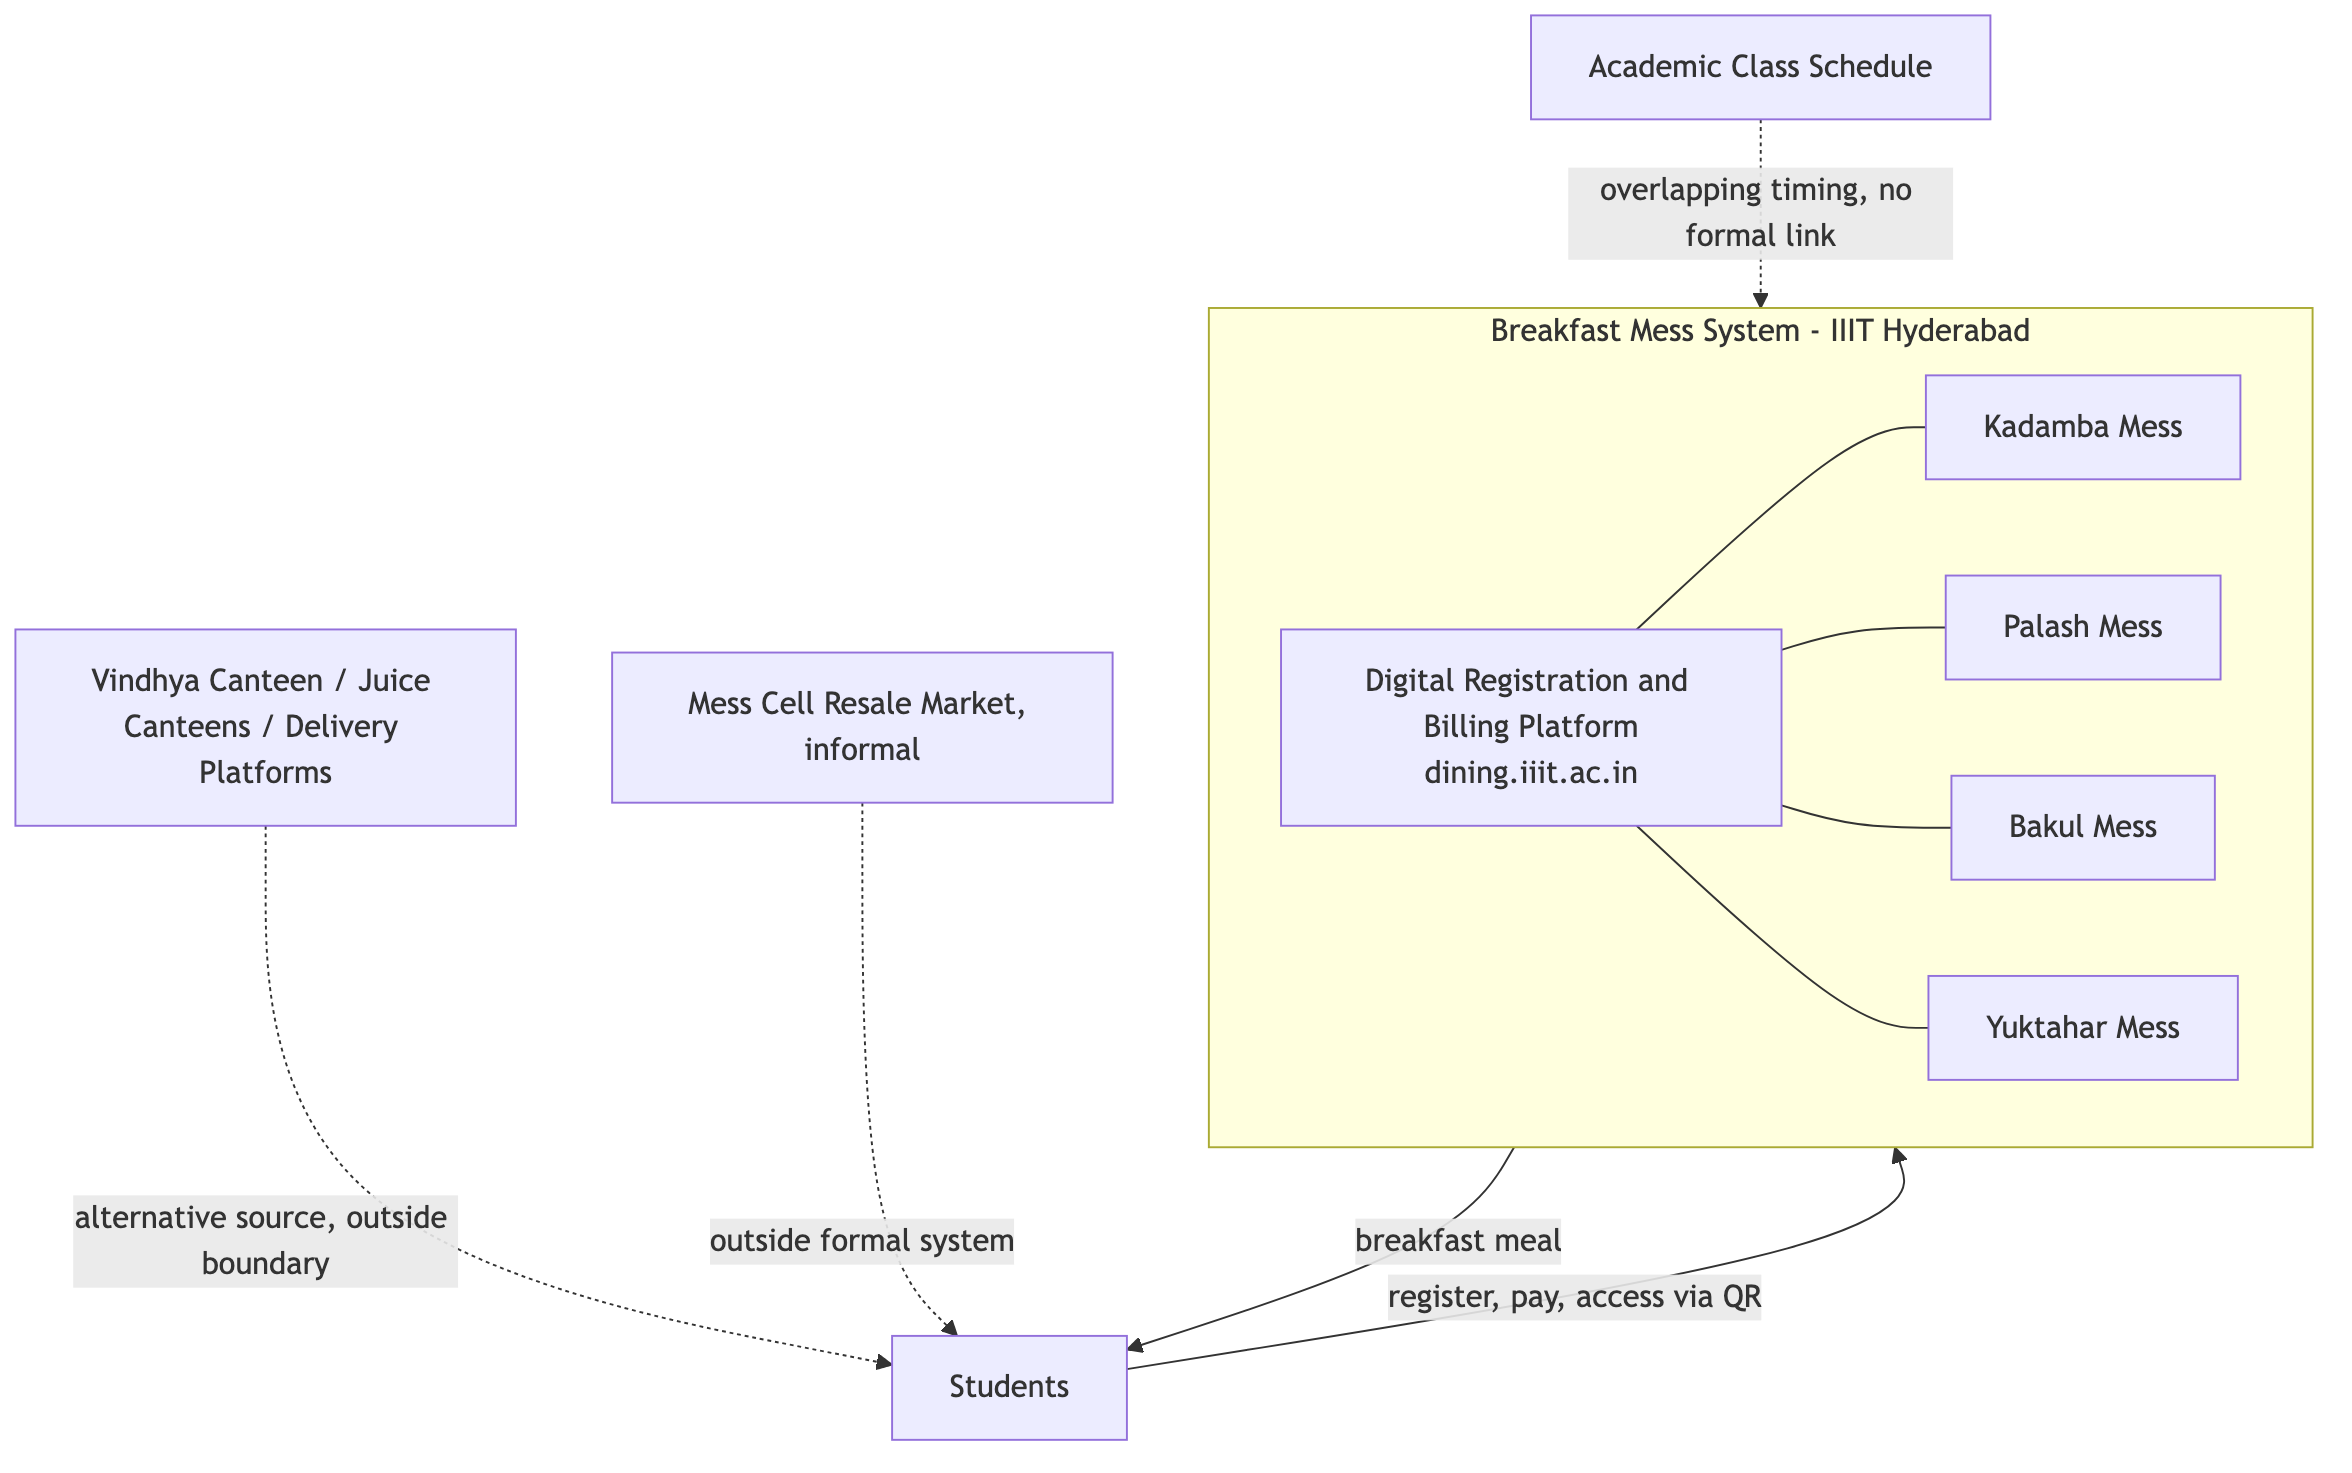
\includegraphics[width=0.85\textwidth]{figures/d1-system-boundary.png}
    \caption{System boundary of the breakfast mess system.}
\end{figure}

\subsection{Context}

The breakfast system serves the entire resident student population of the institute
across four messes, operating daily from 7:30 AM to 9:30 AM. Total confirmed
breakfast capacity across the four messes is approximately 2,755 registrations per
day: Kadamba (700 vegetarian, 600 non-vegetarian), Bakul (350 vegetarian, 350
non-vegetarian), Pal\={a}sh (400), and Yukt\={a}h\={a}r (340 regular, 15 Jain).

Structurally, the system combines centralized demand management with decentralized
supply. A single digital platform governs registration, billing, and access across
all four messes, while food production itself is distributed and non-uniform,
organized around cuisine rather than being interchangeable outlets:

\begin{itemize}
    \item \textbf{Kadamba} --- South Indian food, vegetarian and non-vegetarian; own
        kitchen and vendor.
    \item \textbf{Palash} --- North Indian vegetarian food only; its kitchen cannot
        produce non-vegetarian food at all (a fixed physical limitation, not a policy
        choice).
    \item \textbf{Bakul} --- North Indian food, vegetarian and non-vegetarian: its
        vegetarian food is cooked at Palash and transported to Bakul, while its
        non-vegetarian food is prepared on-site.
    \item \textbf{Yukt\={a}h\={a}r} --- Jain-oriented food, with a separate Jain
        registration variant, operating independently.
\end{itemize}

Food procurement is handled separately by each mess's own vendor, not centrally.
Four different cuisines, kitchens, and procurement arrangements are unified only at
the registration, billing, and access layer --- the mess system is not one kitchen
serving one population through one process, but a coordinated platform sitting over
four structurally different operations.

The system operates inside, and is shaped by, several adjacent systems it does not
control:

\begin{itemize}
    \item \textbf{Academic administration and class schedule.} Classes begin at 8:30
        AM and run until 6:40 PM, with a lunch break from 1:00 PM to 2:00 PM. There is
        no formal channel of coordination between the mess system and the academic
        calendar; the two schedules are set independently by separate authorities.
    \item \textbf{Warden, Mess Committee, and Mess Office governance.} Mess governance
        is split across three actors. The \emph{Mess Committee} is a policy body,
        chaired by a faculty member, that sets the menu and mess-specific policy,
        incorporating student input approximately one month ahead of service. The
        \emph{Mess Office} is the operational arm: it places food orders with each
        vendor on a four-day lead time, administers the registration platform, and
        issues operational policy changes --- a policy change tightening cancellation
        rules was issued by the Mess Office specifically to reduce staff workload. The
        \emph{Warden} holds authority over vendor management and structural changes to
        the mess; the working relationship between the Warden and the Mess Office is
        not established.
    \item \textbf{An informal peer-to-peer resale market (``Mess Cell'').} A WhatsApp
        group has formed in which students who hold a breakfast registration they will
        not use offer it for resale to other students at a negotiated price below the
        registered rate. This market operates entirely outside the mess system's own
        registration and billing infrastructure, transacted through the same personal
        QR-based access credential the formal system issues.
    \item \textbf{The wider campus food ecosystem.} Vindhya Canteen (open Monday to
        Saturday, from 10:00 AM), the juice canteens (open mornings), and delivery
        platforms (accepting orders until 11:00 PM, with delivery personnel required to
        remain outside the campus gate) all draw on the same student population and
        stand as alternatives to mess breakfast.
\end{itemize}

Billing operates on a monthly cycle tied to registration, not attendance: a student is
charged for every meal they are registered for, regardless of whether they eat it, and
may cancel a registration in advance, subject to a limit of five cancellations per meal
type per month. Unregistered (``walk-in'') access to a meal is priced materially higher
than registered access to the same meal.

\begin{figure}[h]
    \centering
    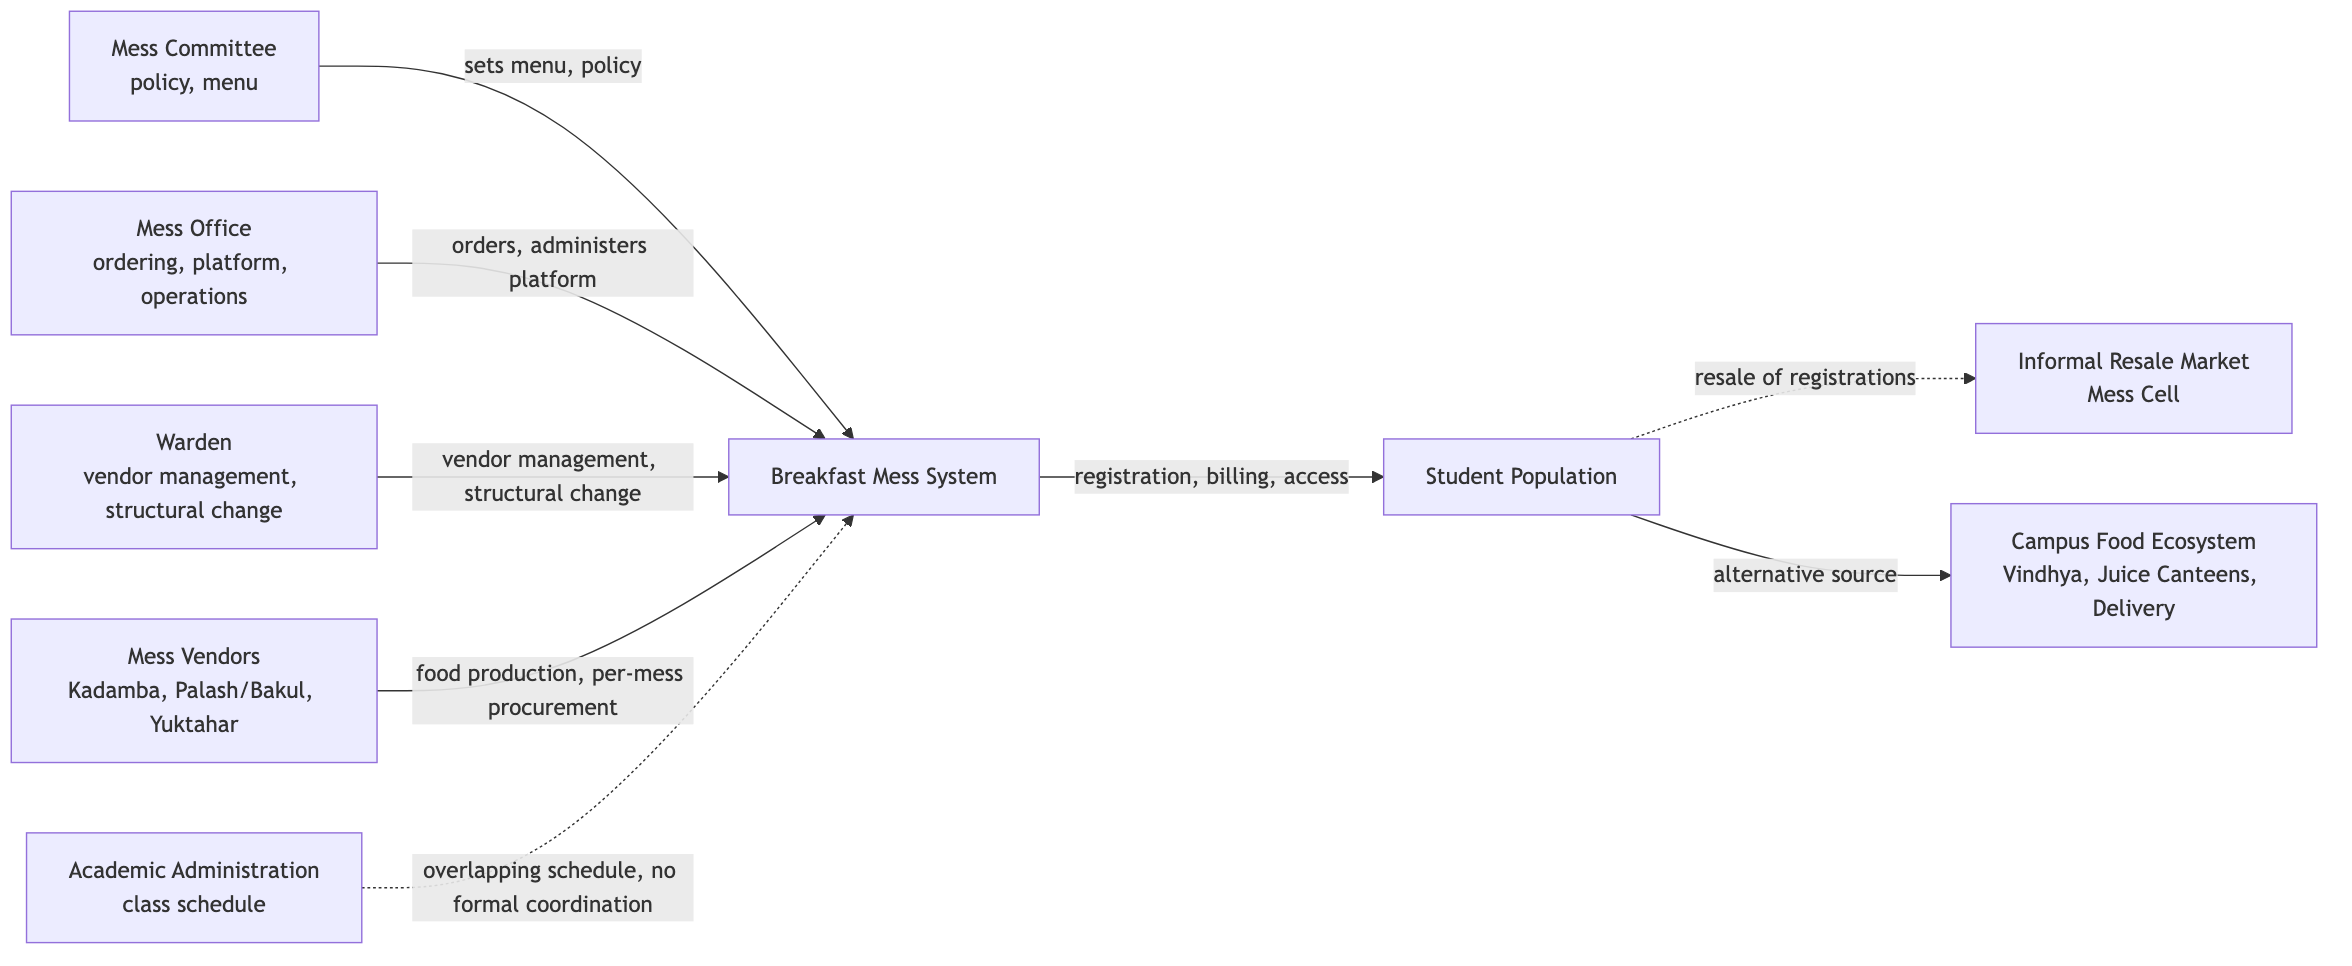
\includegraphics[width=0.85\textwidth]{figures/d2-context-map.png}
    \caption{Context map showing the mess system and the adjacent systems that shape it.}
\end{figure}

\subsection{Purpose and Intended Outcomes}

\textbf{Purpose.} The breakfast mess system exists to provide the resident student
population with reliable, adequate, good-quality food each morning, at a predictable
and affordable cost, accommodating dietary requirements --- vegetarian,
non-vegetarian, and Jain --- in a manner that supports student health, energy, and
academic performance.

\textbf{Intended outcomes.}
\begin{itemize}
    \item Every registered student obtains a breakfast meal matching their dietary
        requirement within the operating window.
    \item Food quality and preparation quantity remain consistent with actual demand,
        minimizing both shortage and waste.
    \item The cost structure remains affordable and predictable for students across a
        full semester.
    \item Access to breakfast does not depend on a student's ability to navigate
        informal workarounds; the formal system functions as the primary and
        sufficient channel on its own.
    \item The system remains responsive to changes in student needs and
        circumstances --- schedule conflicts, dietary changes, feedback --- through
        its own governance structure.
\end{itemize}

\subsection{Visible Symptoms and Underlying Issues}

\begin{longtable}{L{0.45\textwidth}L{0.45\textwidth}}
\toprule
\textbf{Visible Symptom} & \textbf{Underlying Issue} \\
\midrule
\endhead
A student registers for breakfast, does not attend, and is still charged the full
registered price. &
Billing is tied to registration, not attendance. The cost is incurred at the point of
registering, independent of whether the meal is ultimately consumed. \\[6pt]

The registration platform imposes a cap of five cancellations per meal type per
month. &
Uncancelled, unattended registrations occur often enough that an explicit limit was
necessary to manage them --- the cap is itself evidence of the scale of the pattern it
constrains. \\[6pt]

A ``Skip Meal'' function lets a student notify the kitchen in advance of
non-attendance, but this does not reduce or refund the charge. &
The mechanism addresses only the kitchen's production planning, not the student's
cost. It returns zero value to the student for the same situation a cancellation ---
capped at five per month --- would address instead. \\[6pt]

An unofficial, student-run resale market (``Mess Cell'') has formed, where students
sell registrations they will not use to other students. &
Reselling returns partial or full value to the student, while Skip Meal returns none.
For a student who knows in advance they will not attend, resale is a materially
better option than the system's own built-in mechanism. \\[6pt]

Registered-but-unclaimed meals persist despite both a cancellation option and a
resale market being available. &
Cancellation and resale both require advance knowledge of non-attendance.
Last-minute non-attendance --- oversleeping, running out of time, a change of plans
--- has no mechanism available to it at all; this is the category that converts into
prepared, uneaten food with no value returned to anyone. \\[6pt]

Walk-in (unregistered) access to a meal costs substantially more than the same meal
accessed through a prior registration. &
The pricing structure creates a standing incentive to register in advance even when
attendance is uncertain, since deciding same-day costs more. Registration counts are
inflated by this incentive independent of actual intention to attend. \\[6pt]

Registered breakfast attendance is markedly lower, relative to capacity, at every
mess serving North Indian food (Palash, Bakul) than at Kadamba, the South Indian mess
--- Kadamba runs 51--79\% uptake against 11--36.5\% at the North Indian lines. &
The gap tracks cuisine, not any single mess's individual circumstances --- it holds
consistently across three independently operated messes sharing that one variable.
Bakul's status as a newer mess remains a contributing factor, but the cuisine
pattern is the stronger and better-evidenced explanation. \\[6pt]

Neither students nor mess-side staff describe a specific example of mess feedback
leading to a change in policy, hours, or operations. &
Three real channels carry student input into the system --- an in-app per-meal
rating, a public email address, and coverage in \emph{Ping}, the student publication.
None of the three has a confirmed instance of producing a policy change. \\[6pt]

Breakfast hours (7:30--9:30 AM) overlap with the start of the academic day (8:30 AM),
while the two schedules are set by entirely separate authorities. &
Neither side has authority over the other's schedule, and no coordination mechanism
links the two. A timing conflict between them can persist indefinitely without either
side being positioned to resolve it unilaterally. \\[6pt]

The registration platform includes a random-allocation mechanism, evidenced by a
settings option to notify a student when they have been randomly allocated a meal. &
Some registrations are generated by the system itself rather than by active student
choice. Recorded registration counts do not uniformly represent expressed intent to
attend. \\[6pt]

A portion of students report skipping breakfast for reasons unrelated to the mess
system's own operation --- personal dietary practice, sleep schedule, established
habit. &
Breakfast non-attendance is not driven by a single cause; some non-attendance would
persist regardless of any change to mess hours, pricing, or process. \\[6pt]

Students report that companionship affects whether they attend breakfast ---
attendance is more likely when a roommate or friend is also going. &
Breakfast attendance, for at least part of the student population, is a socially
coordinated decision rather than a purely individual one. \\
\bottomrule
\end{longtable}

\subsection{Key Actors, Institutions, Processes, Resources and Constraints}

\subsubsection*{Actors}
\begin{itemize}
    \item \textbf{Students} --- registrants and consumers of the meal; attendance and
        dietary preference vary across the population.
    \item \textbf{Mess Committee} --- a faculty-chaired policy body that sets the menu
        and mess-specific policy.
    \item \textbf{Mess Office} --- the operational and administrative arm; places
        food orders, administers the registration platform, issues operational
        policy changes.
    \item \textbf{Warden} --- holds authority over vendor management and structural
        changes to the mess.
    \item \textbf{Per-mess vendors} --- Kadamba's vendor (South Indian); the shared
        Palash/Bakul vendor (North Indian); Yukt\={a}h\={a}r's vendor (Jain-oriented).
    \item \textbf{Mess serving and cleaning staff} --- also consume mess food after
        student service hours conclude.
    \item \textbf{Academic administration} --- sets the class schedule; holds no
        authority over mess operations.
    \item \textbf{Students participating in the Mess Cell resale market} --- an
        unofficial secondary role occupied by a subset of registered students.
    \item \textbf{Guests} --- parents, visiting relatives, and non-student campus
        affiliates who pay the vendor directly for access.
\end{itemize}

\subsubsection*{Institutions}
The Mess Committee (policy), the Mess Office (operations), and the Office of the
Warden (vendor management and structural change) are three separate governance
actors holding different parts of mess governance. The academic
administration/timetable authority operates independently with no formal link to any
of the three mess-governance actors. The four mess vendors each handle their own
procurement and cooking, operating as independent entities under one shared
registration platform.

\subsubsection*{Processes}
\begin{itemize}
    \item \textbf{Registration} --- a student selects a mess and meal date through the
        digital platform in advance of service.
    \item \textbf{Billing} --- charges are applied monthly, calculated from
        registration count, independent of attendance.
    \item \textbf{Cancellation} --- a registered meal may be cancelled in advance, up
        to five times per meal type per month, removing the associated charge.
    \item \textbf{Skip Meal} --- a registered student may flag in advance that they
        will not attend; this notifies the kitchen for production planning but does
        not affect billing.
    \item \textbf{Access} --- a student presents a personal QR code at the mess
        counter to receive a plate matching their registered dietary category.
    \item \textbf{Walk-in access} --- a student without a registration may pay the
        vendor directly at a higher rate, subject to a separate, smaller capacity
        allocation.
    \item \textbf{Resale} --- outside the formal platform, a registered student may
        transfer their registration to another student through the Mess Cell
        WhatsApp group, in exchange for a negotiated payment.
    \item \textbf{Menu setting} --- the Mess Committee finalizes the menu
        approximately one month ahead of service, incorporating student input.
    \item \textbf{Food ordering} --- the Mess Office places an order with each vendor
        four days ahead of service; vendors prepare food against that four-day-old
        figure, not against same-day registration or cancellation activity.
    \item \textbf{Feedback intake} --- student input reaches the system through an
        in-app per-meal rating, a public email address, and coverage in \emph{Ping};
        none of the three has a confirmed record of producing a resulting policy
        change.
\end{itemize}

\subsubsection*{Resources}
The digital registration and billing platform (\texttt{dining.iiit.ac.in}); four
physical mess facilities of differing capacity and origin --- Kadamba (purpose-built,
largest capacity), Bakul (a converted warehouse), and Palash and Yukt\={a}h\={a}r as
separate facilities; per-mess food production capacity, distributed unevenly by
cuisine; and the personal QR access credential issued to each student.

\subsubsection*{Constraints}
\begin{itemize}
    \item Billing is registration-based, not attendance-based, and cancellations are
        capped at five per meal type per month.
    \item Walk-in pricing is set materially higher than registered pricing.
    \item Vegetarian and non-vegetarian food is segregated by registration type at
        the point of service.
    \item Palash's kitchen cannot produce non-vegetarian food --- a fixed physical
        limitation, not a policy choice.
    \item Mess operating hours and the academic class schedule are set independently
        by separate authorities, with no formal coordination mechanism between them.
    \item Governance authority over mess operations is split across the Mess
        Committee, the Mess Office, and the Warden; the academic administration has
        no formal role in mess-related decisions.
    \item Vendors order and prepare food against a four-day-old registration figure;
        nothing in the system lets same-day registration, cancellation, or Skip Meal
        activity change what is actually cooked.
\end{itemize}

\subsection{Initial Problem Framing}

Many students register for breakfast and do not eat it. The meal is still cooked, and
the student is still charged.

The system gives students two ways to avoid this: cancel the registration, or mark it
as skipped. Skip Meal returns no money to the student --- only cancellation does, and
only five times a month per meal. Both require the student to decide in advance. A
student who decides at the last minute has no option at all, and that meal is simply
wasted. Students have built their own workaround outside the system --- reselling
registrations to each other --- because it pays back more than the system's own tools
do.

\begin{quote}
\textbf{The problem:} registration does not reliably reflect who is actually going to
eat. Why not, and what in the system is causing that gap?
\end{quote}

\newpage

%============================================================
\section{Task 2: Stakeholder Map}
\status{Complete}

\subsection{Use Case}

The breakfast mess system at IIIT Hyderabad registers, bills, and serves breakfast to
the resident student population across four messes --- Kadamba, Palash, Bakul, and
Yukt\={a}h\={a}r --- through a single digital platform. Registration counts, not
attendance, drive billing and food procurement. This map identifies every actor,
institution, and informal structure that participates in, influences, benefits from,
or is affected by this system, and the relationships, dependencies, and conflicts
between them.

Twenty-seven candidate actors were identified across seventeen analytical lenses
(student/user, social, food production, governance, money, technology, academic,
sleep/time-use, substitute systems, campus infrastructure, waste, health, policy,
informal systems, absent/sleeping stakeholders, temporal, and intervention).
Seventeen were included in the final map; four were treated as minor rather than
included in full; three were considered and excluded entirely (a campus
health/wellbeing office, senior-to-junior norm transmission, and a parental financial
relationship, since mess fees are bundled into hostel fees).

\subsection{Primary, Secondary, and Indirect Stakeholders}

\textbf{Primary stakeholders} --- direct, daily interaction with the system:

\begin{longtable}{L{0.55\textwidth}L{0.35\textwidth}}
\toprule
\textbf{Stakeholder} & \textbf{Type} \\
\midrule
\endhead
Students & Human group --- registrant, billed party, consumer \\
Vendor --- South Indian (Kadamba) & Commercial \\
Vendor --- North Indian (Palash veg-only + Bakul veg/non-veg) & Commercial \\
Vendor --- Jain (Yukt\={a}h\={a}r) & Commercial \\
Mess serving/counter staff & Human group \\
Kitchen/cooking staff & Human group \\
\bottomrule
\end{longtable}

\textbf{Secondary stakeholders} --- govern, execute, or manage the system without
daily direct interaction:

\begin{longtable}{L{0.55\textwidth}L{0.35\textwidth}}
\toprule
\textbf{Stakeholder} & \textbf{Type} \\
\midrule
\endhead
Mess Committee & Institution --- policy \\
Mess Office & Institution --- operations \\
Warden & Individual role --- vendor management, structural change \\
\bottomrule
\end{longtable}

\textbf{Indirect stakeholders} --- affected by or connected to the system without
direct engagement, including latent (``sleeping'') actors currently inert but
holding potential leverage:

\begin{longtable}{L{0.55\textwidth}L{0.35\textwidth}}
\toprule
\textbf{Stakeholder} & \textbf{Type} \\
\midrule
\endhead
Academic administration / timetable authority & Institution --- latent \\
Facilities/Estate team & Institution --- latent \\
Portal/IT system owner & Institution or individual --- latent \\
Mess Cell WhatsApp community & Informal group \\
Unofficial mess-tool developers & Individual(s) --- latent \\
Ping (student publication) & Institution --- latent \\
Vindhya Canteen and juice canteens & Commercial --- substitute \\
Delivery platforms and riders & Commercial --- substitute \\
\bottomrule
\end{longtable}

\subsection{Stakeholder Interests, Needs, and Expectations}

{\small\setlength{\tabcolsep}{4pt}
\begin{longtable}{L{0.19\textwidth}L{0.23\textwidth}L{0.23\textwidth}L{0.21\textwidth}}
\toprule
\textbf{Stakeholder} & \textbf{Interest} & \textbf{Need} & \textbf{Expectation} \\
\midrule
\endhead
Students & Convenient, affordable, timely food; not paying twice for a missed meal &
A functioning registration/billing system, predictable hours, food matching dietary
registration & Registering reliably results in being fed; being charged regardless
of attendance is tolerated, not agreed \\[4pt]

Vendor --- Kadamba (South Indian) & Contract renewal, predictable order volume,
margin & An accurate registration forecast, currently four days ahead & The four-day
forecast approximates real demand \\[4pt]

Vendor --- Palash + Bakul (North Indian) & Contract renewal, predictable order
volume, margin & Same four-day lead time; Palash cannot produce non-veg food, a fixed
limitation & Demand for the veg line cooked at Palash and transported to Bakul stays
predictable \\[4pt]

Vendor --- Yukt\={a}h\={a}r (Jain) & Contract renewal, predictable order volume,
margin & Same four-day lead time; relationship to other vendors unconfirmed & Same as
other vendors \\[4pt]

Serving and kitchen staff & Manageable preparation and service load, predictable
headcounts & Sufficient lead time and an accurate registration count & Leftover food
is theirs to consume after service hours --- an informal norm \\[4pt]

Mess Committee & Balancing student satisfaction against operational feasibility & A
functioning process for gathering and interpreting student input & The existing
menu-input process constitutes sufficient engagement on mess matters generally \\[4pt]

Mess Office & Reduced operational workload --- its stated motive for its one
confirmed policy change & An accurate same-day picture of intent, currently
unavailable at less than four days' notice & Registration counts are a workable
proxy for actual attendance \\[4pt]

Warden & Stable vendor relationships, orderly mess infrastructure & Clear division of
responsibility with the Mess Office & Vendor management and structural authority
remain within the Warden's own lane \\[4pt]

Academic administration & Its own domain --- class scheduling --- run without
external interference & No stated need connects it to mess operations & No
expectation of any relationship to mess governance \\[4pt]

Facilities/Estate team & Physical infrastructure upkeep & Authorization and budget
for mess-facility work & Not established --- identity of this actor is itself
unconfirmed \\[4pt]

Portal/IT system owner & System uptime and reliability of the registration interface
& Not established & Not established --- no source names this actor \\[4pt]

Mess Cell WhatsApp community & Recovering value from a registration that will go
unused & A way to transfer a registration since Skip Meal returns no money & Buyers
and sellers can find each other informally and transact on trust \\[4pt]

Unofficial mess-tool developers & Not established beyond building the tool itself &
Not established & Described as built ``for students of IIIT Hyderabad'' \\[4pt]

Ping (student publication) & Reporting on mess issues as a matter of student interest
& Access to information worth publishing & Not established whether coverage produces
institutional response \\[4pt]

Vindhya Canteen and juice canteens & Capturing demand when mess breakfast is skipped
or unavailable & Steady walk-in customer flow & Not established \\[4pt]

Delivery platforms and riders & Capturing demand when mess breakfast is skipped or
unavailable & Gate access for delivery, currently restricted & Not established \\
\bottomrule
\end{longtable}}

\subsection{Formal and Informal Roles}

\textbf{Formal roles} attach to every institutional and commercial actor: Students
(as registrant), Mess Committee, Mess Office, Warden, the three vendors, serving and
kitchen staff, Vindhya Canteen and juice canteens, and delivery platforms all hold a
formal, rule-defined position in the system.

\textbf{Informal roles} attach to the Mess Cell WhatsApp community, Ping, and the
unofficial mess-tool developers --- none of these has any official standing in the
system, yet each performs a real function (resale market, public-pressure channel,
and an alternative registration interface, respectively).

\textbf{Roles that are not separate stakeholders.} Several categories that might
appear as distinct actors are, on inspection, behavioral states or temporary roles
occupied by the single actor Students, not separate stakeholders in their own right:
attending regularly, skipping regularly, having an early class on a given day, buying
or selling on Mess Cell, and using an unofficial registration tool are all states a
single student may move through within the same week. Peer influence between
students is an internal relationship on the Students node, not a separate
``Friends'' or ``Roommates'' stakeholder. Guest diners are the one genuine exception:
they hold a materially different formal relationship, but their volume is too
marginal to warrant inclusion as a full stakeholder.

\subsection{Stakeholder Maps}

\begin{figure}[h]
    \centering
    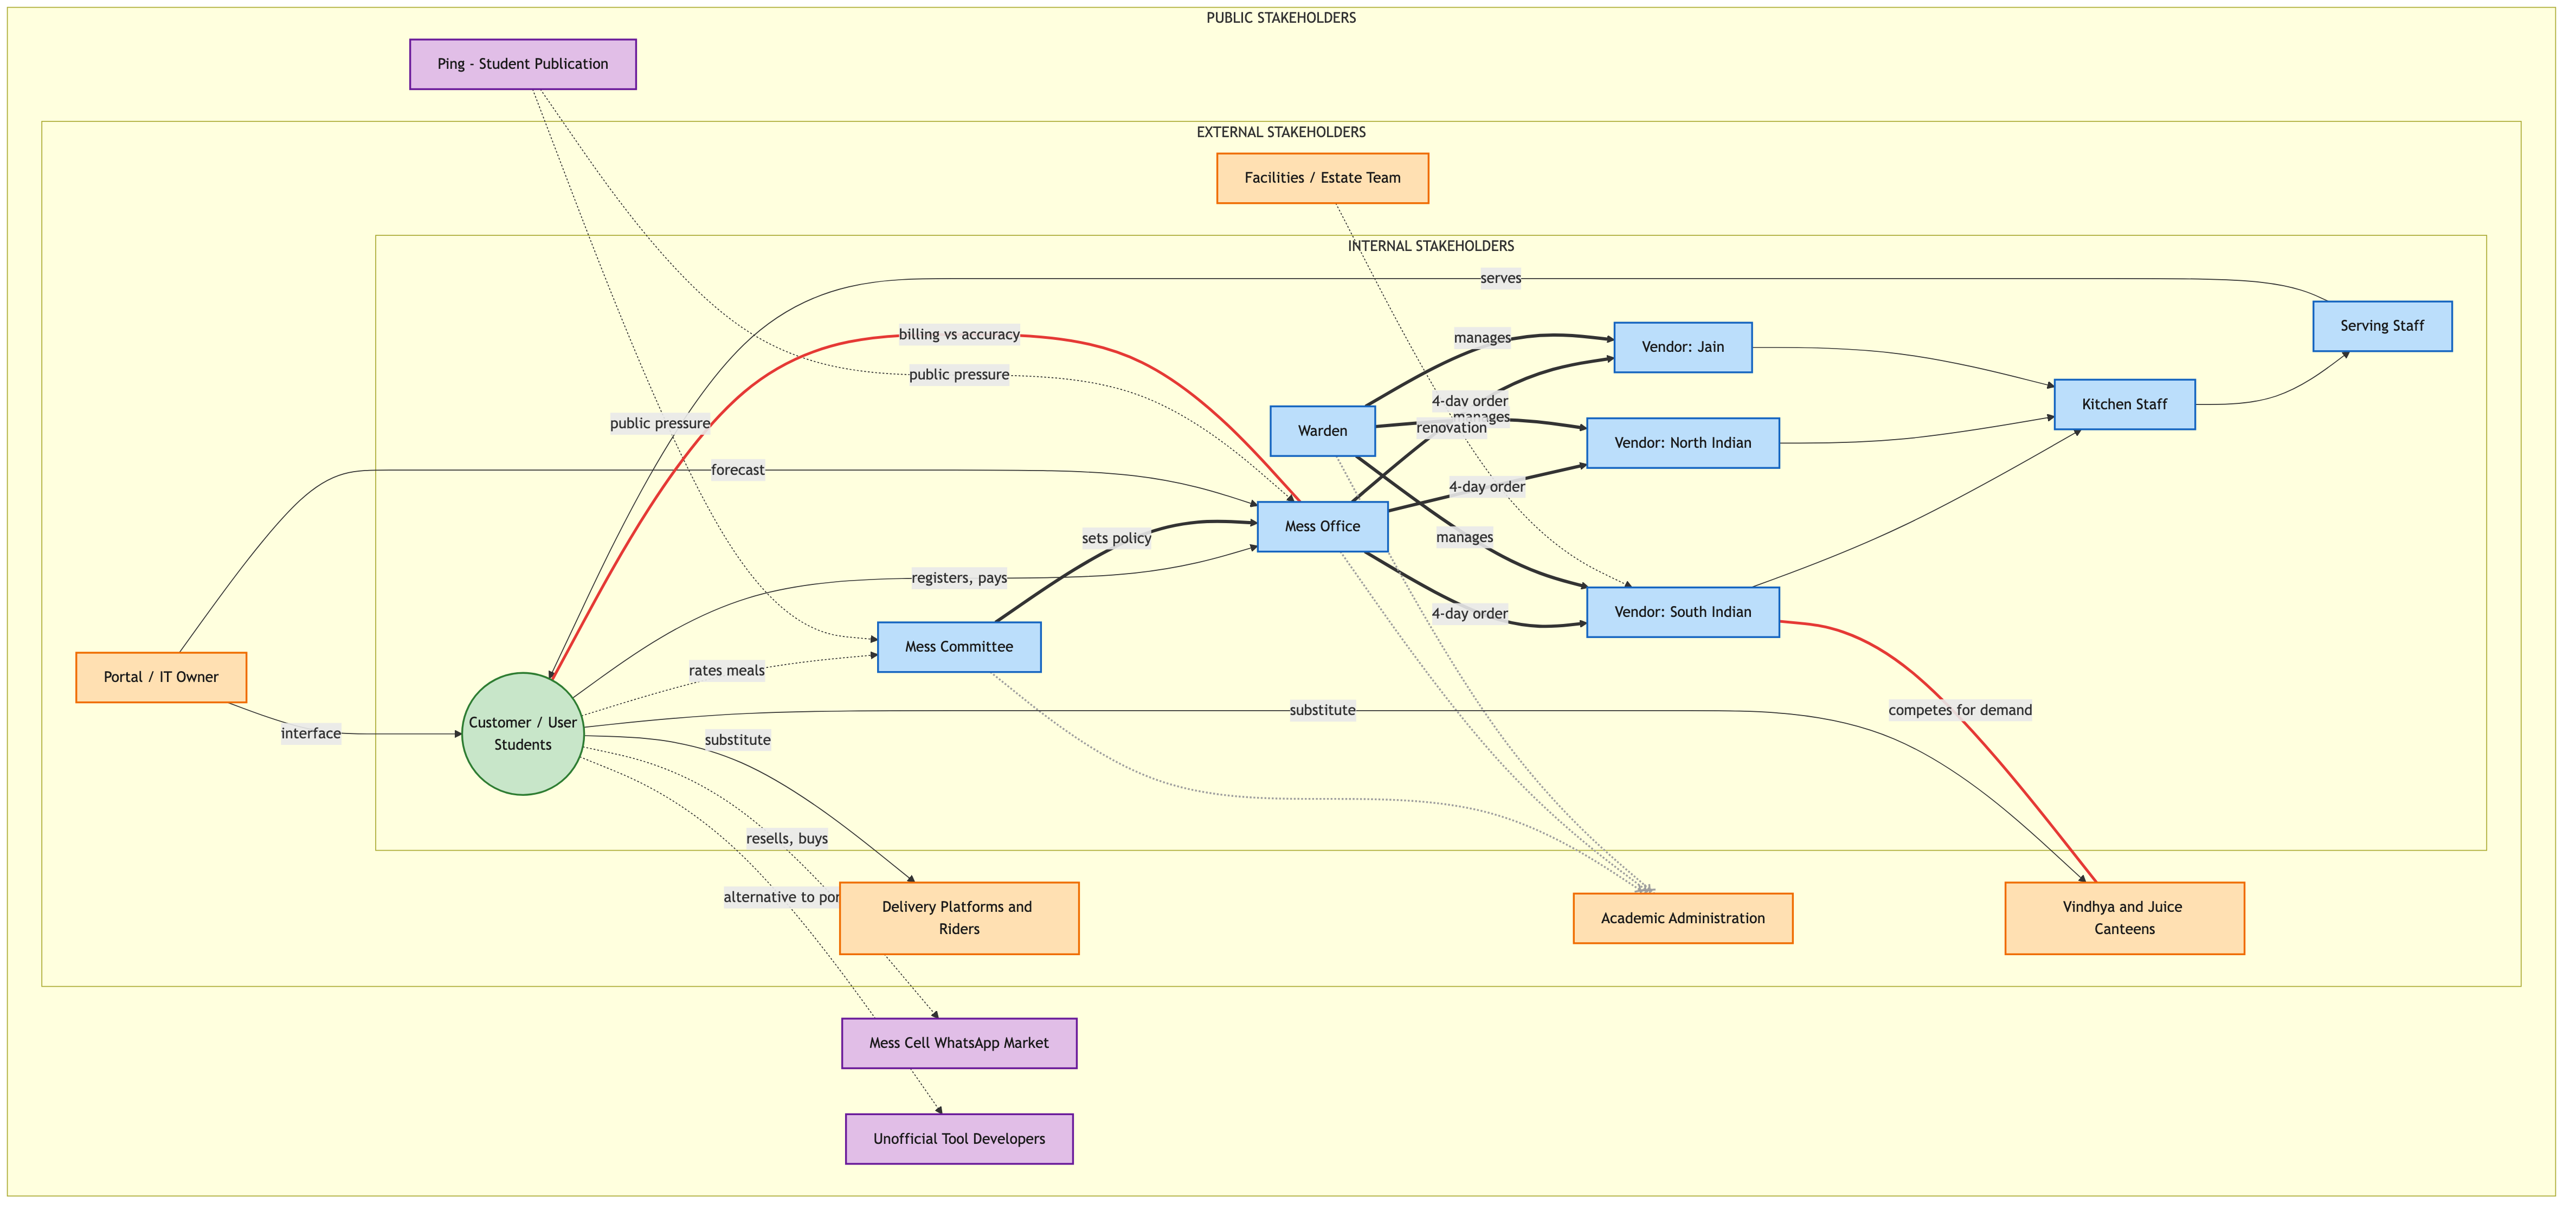
\includegraphics[width=0.9\textwidth]{figures/d3-stakeholder-map.png}
    \caption{Stakeholder map, placed by the standard four-ring model (customer/user,
    internal, external, public).}
\end{figure}

\begin{figure}[h]
    \centering
    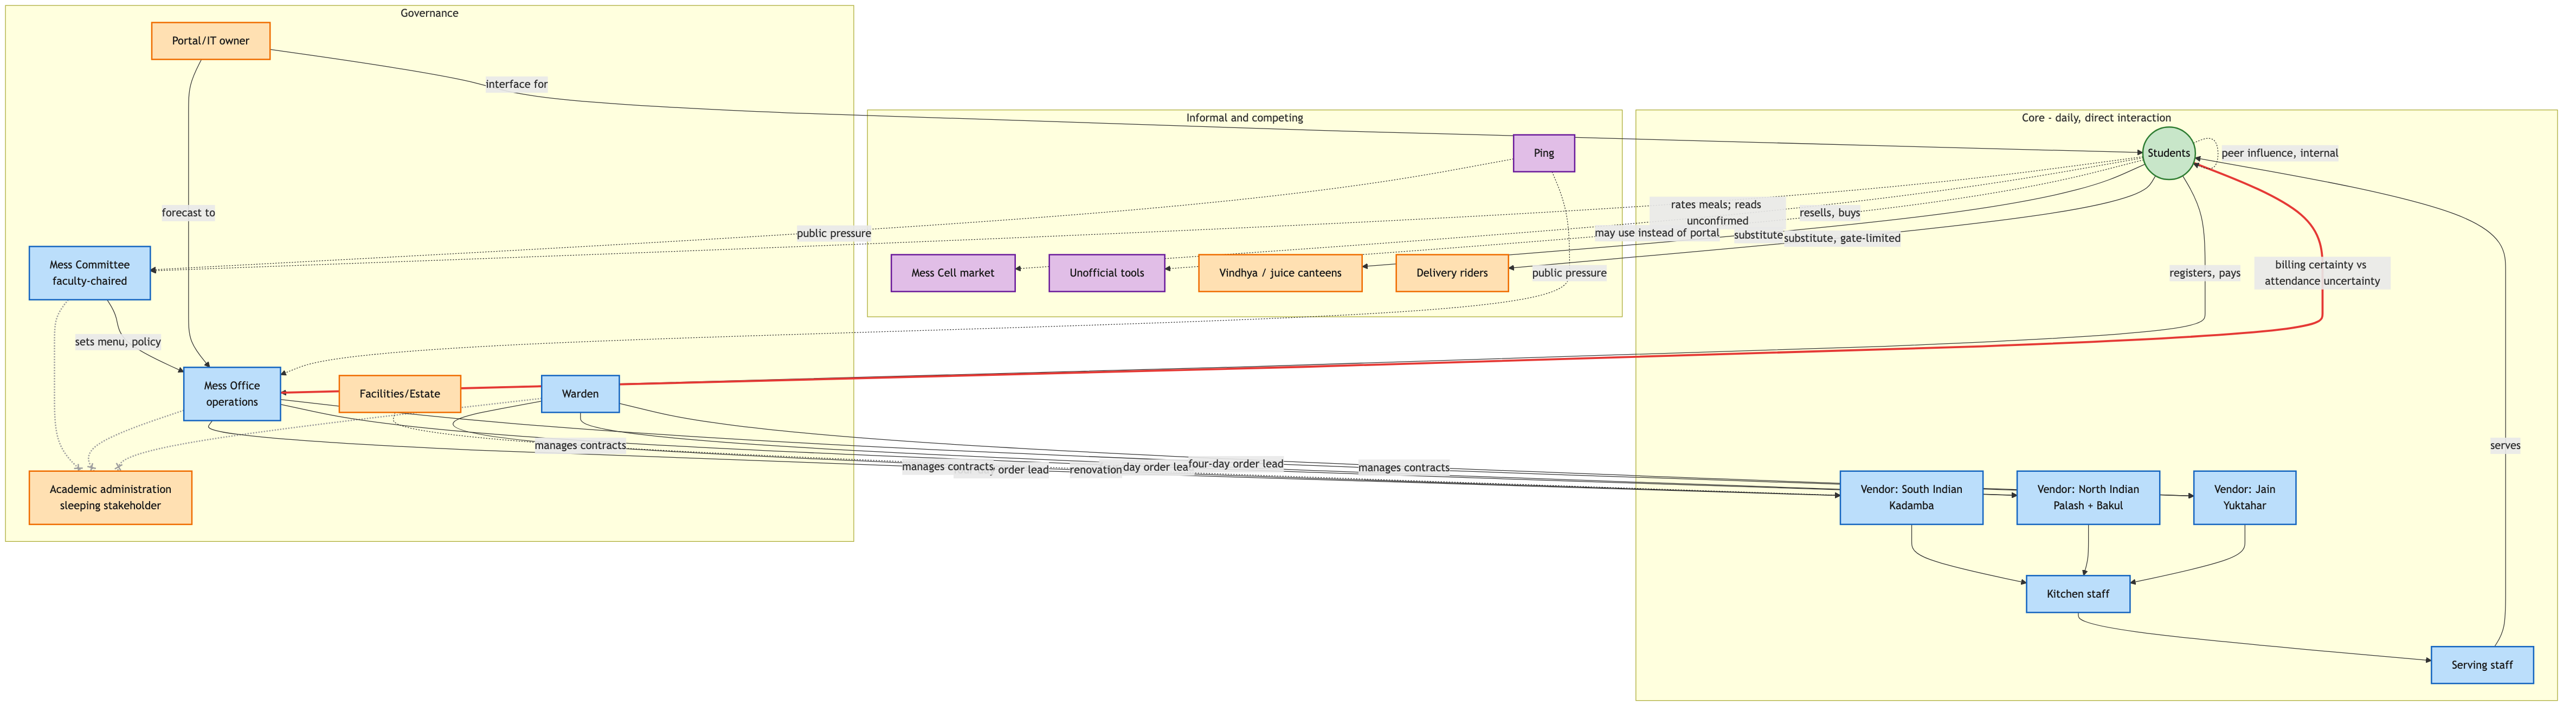
\includegraphics[width=0.9\textwidth]{figures/d4-relationship-network.png}
    \caption{Relationship network --- the same seventeen stakeholders laid out by
    functional cluster (core daily operation, governance, informal/competing).}
\end{figure}

\begin{figure}[h]
    \centering
    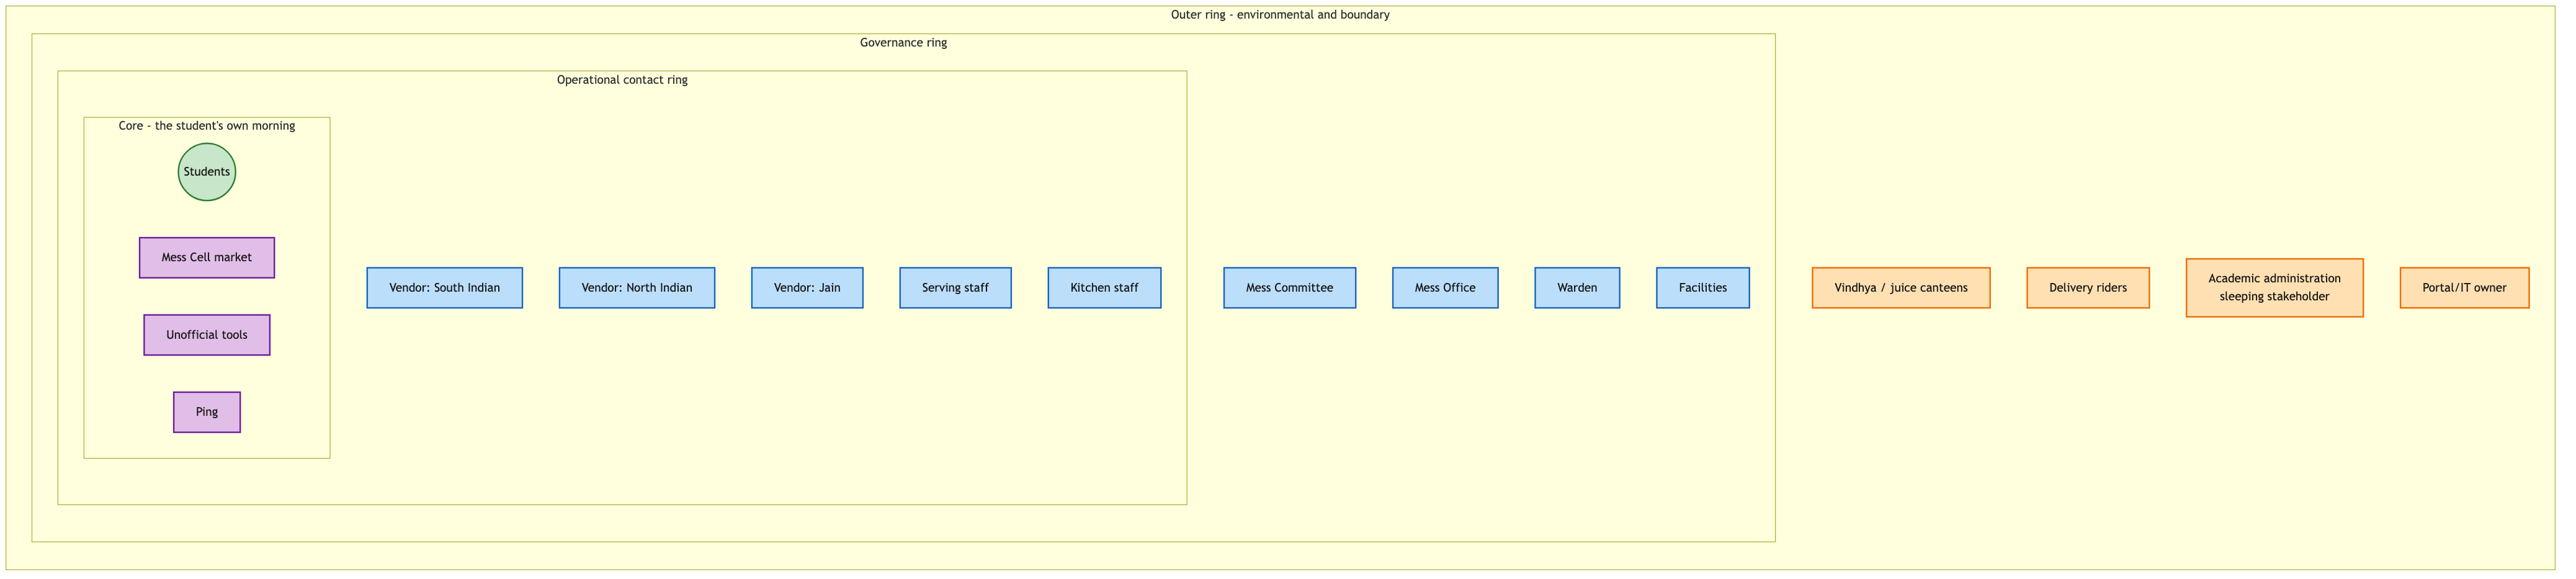
\includegraphics[width=0.75\textwidth]{figures/d5-onion-proximity.png}
    \caption{Onion proximity map --- stakeholders clustered by closeness to a
    student's actual morning rather than by relationship type. Academic
    administration sits at the outermost ring with no adjacent inward relationship at
    any layer, while Mess Cell, unofficial tools, and Ping sit at the innermost ring
    alongside the students themselves.}
\end{figure}

\subsection{Relationships, Dependencies, and Conflicts}

\subsubsection*{Relationship matrix}

Cells marked \hypo\ have not been independently confirmed.

{\small\setlength{\tabcolsep}{3pt}
\begin{longtable}{L{0.13\textwidth}L{0.155\textwidth}L{0.155\textwidth}L{0.155\textwidth}L{0.14\textwidth}L{0.155\textwidth}}
\toprule
 & \textbf{Students} & \textbf{Mess Committee} & \textbf{Mess Office} & \textbf{Warden} & \textbf{Vendors} \\
\midrule
\endhead
\textbf{Students} & --- & Feedback (rating system confirmed; whether read is
unconfirmed) & Registration, payment & --- & Payment, service \\[4pt]
\textbf{Mess Committee} & Authority (menu, feedback) & --- & Authority (sets policy)
& \hypo\ overlap & Authority (menu) \\[4pt]
\textbf{Mess Office} & Billing; dependent on for order accuracy & Reports to
(\hypo) & --- & \hypo\ overlap & Authority, dependency (ordering) \\[4pt]
\textbf{Warden} & --- & \hypo & \hypo & --- & Authority (contracts) \\[4pt]
\textbf{Vendors} & Payment, food/material & Authority over & Authority over,
dependency & Contract authority & --- \\
\bottomrule
\end{longtable}}

Academic administration has no confirmed relationship of any kind to any of the
three governance actors --- a genuine structural gap, not a modeling omission, and
the single most consequential finding in this map.

\subsubsection*{Dependencies}

Students depend on vendors for food quality and timing; vendors do not depend on any
individual student --- an asymmetric dependency consistent with a walk-in pricing
structure that requires no negotiation. Vendors depend on the Mess Office for a
registration forecast fixed four days ahead of service; the Mess Office depends on
students to register accurately, but nothing in the billing structure requires
accuracy, since a student is charged identically whether or not they attend --- the
weakest link in this dependency chain is also the one with no incentive attached to
it.

The Mess Committee depends on the Mess Office to execute policy; the Mess Office's
own stated motivation for its one confirmed policy change (reducing workload) did
not visibly originate from or require Mess Committee direction, suggesting
operational pressure may drive policy from below at least as often as governance
drives it from above.

No source describes a direct relationship between vendors and students --- all
communication routes through the Mess Office or the portal. No source describes the
Portal/IT owner having any direct relationship with the Mess Committee, despite the
Committee setting policy this system presumably enforces technically.

\subsubsection*{Conflicts}

\begin{longtable}{L{0.28\textwidth}L{0.33\textwidth}L{0.33\textwidth}}
\toprule
\textbf{Conflict} & \textbf{Side A} & \textbf{Side B} \\
\midrule
\endhead
Billing certainty vs.\ attendance uncertainty & Mess Office and vendors need a
stable number to order against, fixed four days ahead & Students face genuinely
uncertain day-to-day attendance, with no incentive built into billing to report it
accurately \\[6pt]

Flexibility vs.\ workload & Students and the Mess Cell market want more
cancellation and resale flexibility & The Mess Office's one confirmed policy change
tightened rules specifically to reduce staff workload \\[6pt]

Convenience vs.\ waste & Students want flexible registration & The Mess Office wants
predictable, low-workload ordering \\[6pt]

Cuisine demand vs.\ fixed procurement & Registered uptake is markedly lower at every
North Indian line (Palash, Bakul) than the South Indian line (Kadamba) & The four
cuisine lines are fixed by vendor contract, not adjusted in response to demand \\[6pt]

Academic schedule vs.\ meal schedule & Academic administration owns class timing and
holds no stake in mess outcomes & Students bear the actual cost of the 8:30 AM
overlap with breakfast hours \\
\bottomrule
\end{longtable}

\subsection{Findings}

Twenty-seven candidate stakeholders were narrowed to seventeen through direct
evidence rather than assumption. The Mess Office is a distinct actor from the Mess
Committee, separating ``who decides policy'' from ``who executes it'' --- every
earlier account of this system's governance, including this team's own first drafts,
had collapsed the two into one.

Academic administration holds the single lever most likely to materially affect the
core problem --- the overlap between breakfast hours and the 8:30 AM class start ---
and has no relationship of any kind, formal or informal, to any of the three
mess-governance actors. This is the clearest sleeping stakeholder in the map: total
authority over the one variable in conflict, zero engagement with the system it
conflicts with.

Three real feedback channels exist --- an in-app per-meal rating, a public email
address, and coverage in \emph{Ping} --- and none has a confirmed instance of
producing a policy change. Inputs exist; a confirmed output does not.

Registered attendance is markedly lower, relative to capacity, at every mess serving
North Indian food than at the South Indian mess, a pattern consistent across three
independently operated messes, making cuisine preference a stronger candidate
explanation for the uptake gap than any single mess's individual circumstances.

The Mess Committee's faculty chair is a second, more subtle sleeping stakeholder: an
individual with cross-institutional standing that no student-only channel possesses,
and the most structurally plausible bridge to Academic administration available, with
no evidence that bridge has ever been used.

Two structurally hidden actors carry outsized influence without being visible to any
single respondent: the Portal/IT system owner, interacted with constantly and named
by no one, and the four-day procurement lead time itself --- not a person, but a
fixed constraint that caps how responsive the entire system can be to any same-day
signal, including Skip Meal.

\newpage

%============================================================
\section{Task 3: Stakeholder Power--Interest / Leverage Map}
\status{Draft --- built from confirmed context-brief and stakeholder-map facts; to be finalized once governance-side (Role D) interview data lands}

\subsection{Power Analysis Brief}

Power is defined as decision-making authority plus resource control. Interest is how
much the outcome affects the actor, or how much attention they actually pay it ---
these are not always the same thing, as the Academic Office row below shows.

{\small
\begin{longtable}{L{0.19\textwidth}L{0.27\textwidth}L{0.15\textwidth}L{0.22\textwidth}}
\toprule
\textbf{Actor} & \textbf{Power} & \textbf{Interest} & \textbf{Quadrant} \\
\midrule
\endhead
Mess Committee & High --- sets menu/rules & High & Manage Closely \confirmed \\[4pt]
Warden & High --- vendor management, structural changes & Medium-High & Manage
Closely \confirmed \\[4pt]
Per-mess vendors/catering providers & Medium-High --- controls supply
volume/quality/cost & Medium & Manage Closely / Keep Satisfied \hypo \\[4pt]
Academic Office / timetable authority & High --- controls the one lever (class
start time) that could resolve the core paradox & Very Low --- no mandate/attention
on mess matters & Nominally ``Keep Satisfied'', functionally disengaged --- a
\textbf{sleeping power} \hypo \\[4pt]
Students & Low --- no formal decision authority, ``input'' only & Very High ---
bears cost and experience directly & Keep Informed --- a textbook mismanaged
quadrant \confirmed/\hypo \\[4pt]
Mess serving/kitchen/cooking staff & Low formal power --- execute decisions & High
--- workload, waste, day-to-day friction & Keep Informed --- an underused source of
operational truth \hypo \\[4pt]
Mess Cell WhatsApp community & None formal, but high de facto structural influence
(absorbs waste/no-show pressure the official system doesn't handle) & High &
Monitor formally / arguably deserves Manage Closely once its real scale is known
\hypo \\[4pt]
Vindhya/juice canteens, delivery riders & Low power over the mess system itself &
Medium --- business interest in capturing skippers & Monitor \confirmed \\[4pt]
Friends/Roommates & Low power at system level & High interest at the
individual-decision level, not systemic & Out of formal power--interest scope ---
relevant to the Process Trace instead \hypo \\
\bottomrule
\end{longtable}}

\subsection{Quadrant Chart}

\begin{figure}[h]
    \centering
    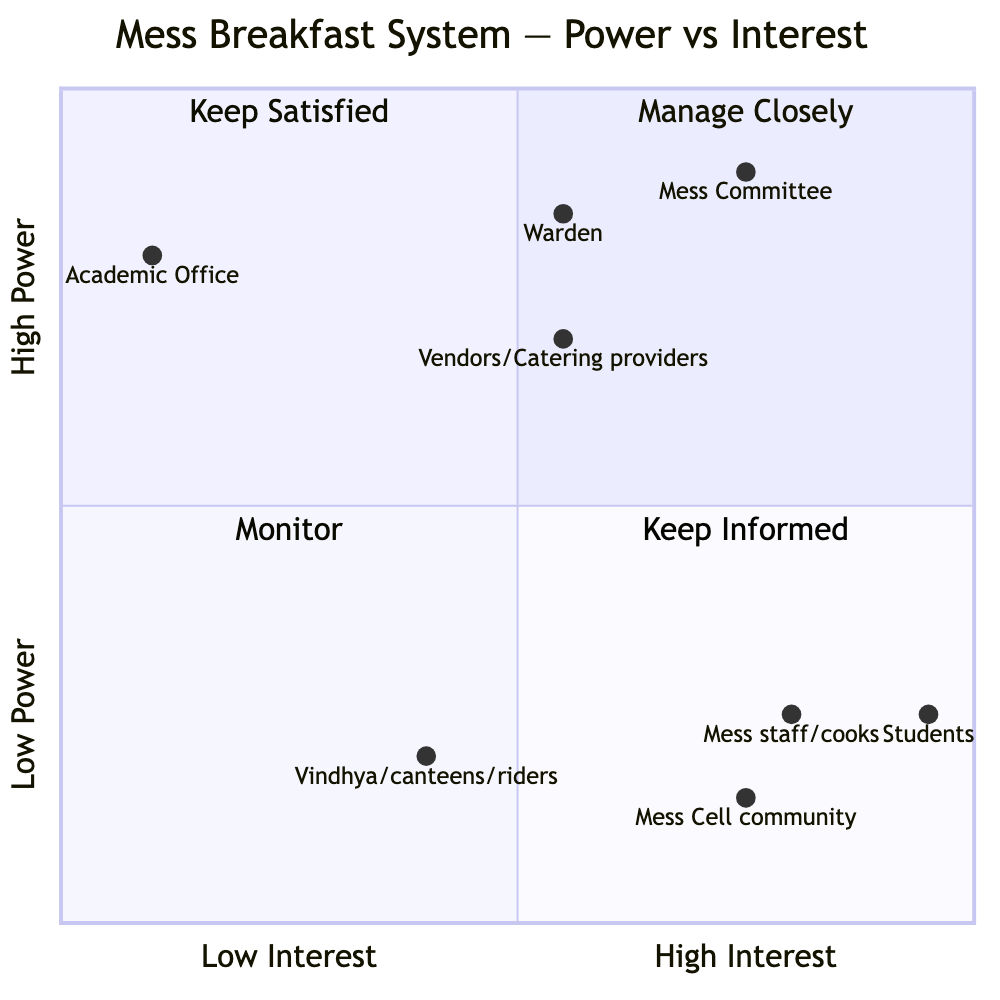
\includegraphics[width=0.8\textwidth]{figures/d6-power-interest.png}
    \caption{Power--Interest quadrant chart for the mess breakfast system.}
\end{figure}

\subsection{Strategic Findings}

\begin{enumerate}
    \item \textbf{Academic Office is a ``sleeping power.''} It holds the single lever
        most likely to resolve the core paradox --- shifting the 8:30 AM class start,
        or even just the first class of the week --- but has no interest or mandate
        that would make it act. This is a structural / mental-model finding to carry
        into the Phase 2 Iceberg analysis, not just a gap in the map.
    \item \textbf{Mess staff are high-interest, near-zero-formal-power}, and their
        operational knowledge (waste volume, real headcounts, cost/workload pressure)
        does not appear to reach decision-makers through any formal channel. The
        mess-staff (Role C) interview is as much a data point for this map as it is
        for the Process Trace.
\end{enumerate}

\subsection{Open Items --- to be closed by interviews}

\begin{itemize}
    \item Confirm the real scale/frequency of Mess Cell activity --- would move it
        from ``Monitor'' toward ``Manage Closely'' if larger than assumed.
    \item Confirm students' own sense of their interest/power (currently plotted
        from the context brief's structural facts, not from a student's own framing).
    \item Confirm the vendor vs.\ catering-provider power split once staff interviews
        clarify which messes use which model.
\end{itemize}

\newpage

%============================================================
\section{Task 4: Current-State Process Map / Process Trace}
\status{Draft --- awaiting real interview and observation data (Activity 4 explicitly requires ``interviews and observations''); everything below is the best-effort scaffold to be corrected, not a result to cite}

\subsection{Why a Process Trace, Not Just a Stakeholder Map}

The stakeholder map says \emph{who} is involved. This section is supposed to say
\emph{what actually happens}, step by step, including the workarounds --- per the
framework's own phrasing, ``how the system actually operates rather than how it is
supposed to operate.'' The gap between those two is exactly where the Breakfast
Paradox lives: the \emph{designed} process is register $\rightarrow$ attend
$\rightarrow$ eat; the \emph{actual} process, per every account gathered so far, has
several parallel exit ramps around ``attend.''

Confirmed context-brief facts describe billing and cancellation at the
\emph{monthly} level, but a plausible \emph{weekly} registration habit may sit on
top of the \emph{daily} attendance decision --- three different timescales that a
single word, ``process,'' can hide if traced as only one loop.

\subsection{A. Weekly Cycle}
\hypo\ Unconfirmed by any real respondent yet.

\begin{figure}[h]
    \centering
    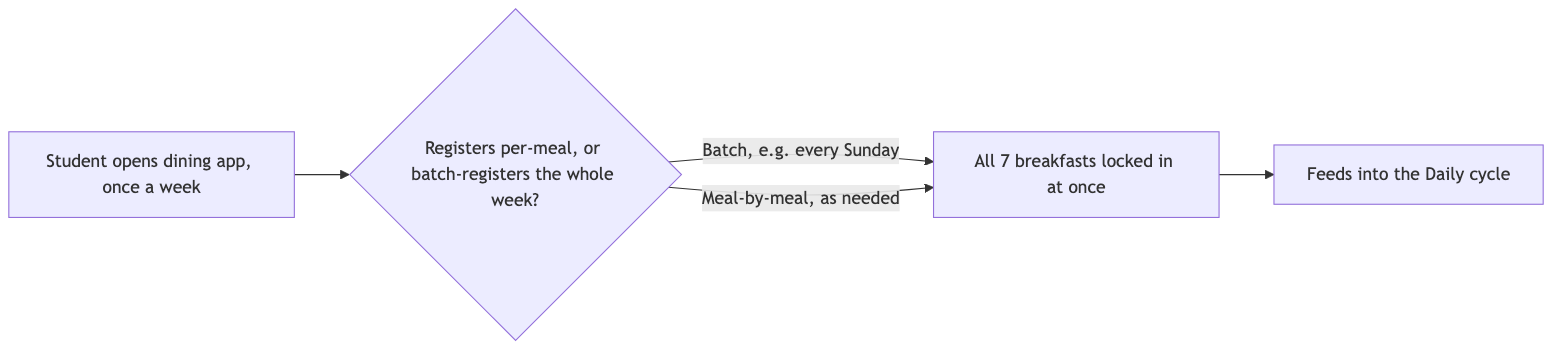
\includegraphics[width=0.85\textwidth]{figures/d7-weekly-cycle.png}
    \caption{Weekly registration cycle (hypothesis).}
\end{figure}

If a batch-registration pattern (registering for the whole week at once, rather than
meal-by-meal) is real and common, it mechanically decouples the registration
decision from the morning-of attendance decision --- a student who registers Sunday
for Wednesday is not ``deciding to eat Wednesday,'' they are deciding once for the
whole week. This would explain a large share of the no-show volume without any
single morning being anyone's fault, and is the single highest-value hypothesis to
confirm through direct interview.

\subsection{B. Daily Cycle (7:30--9:30 AM window)}

\begin{figure}[h]
    \centering
    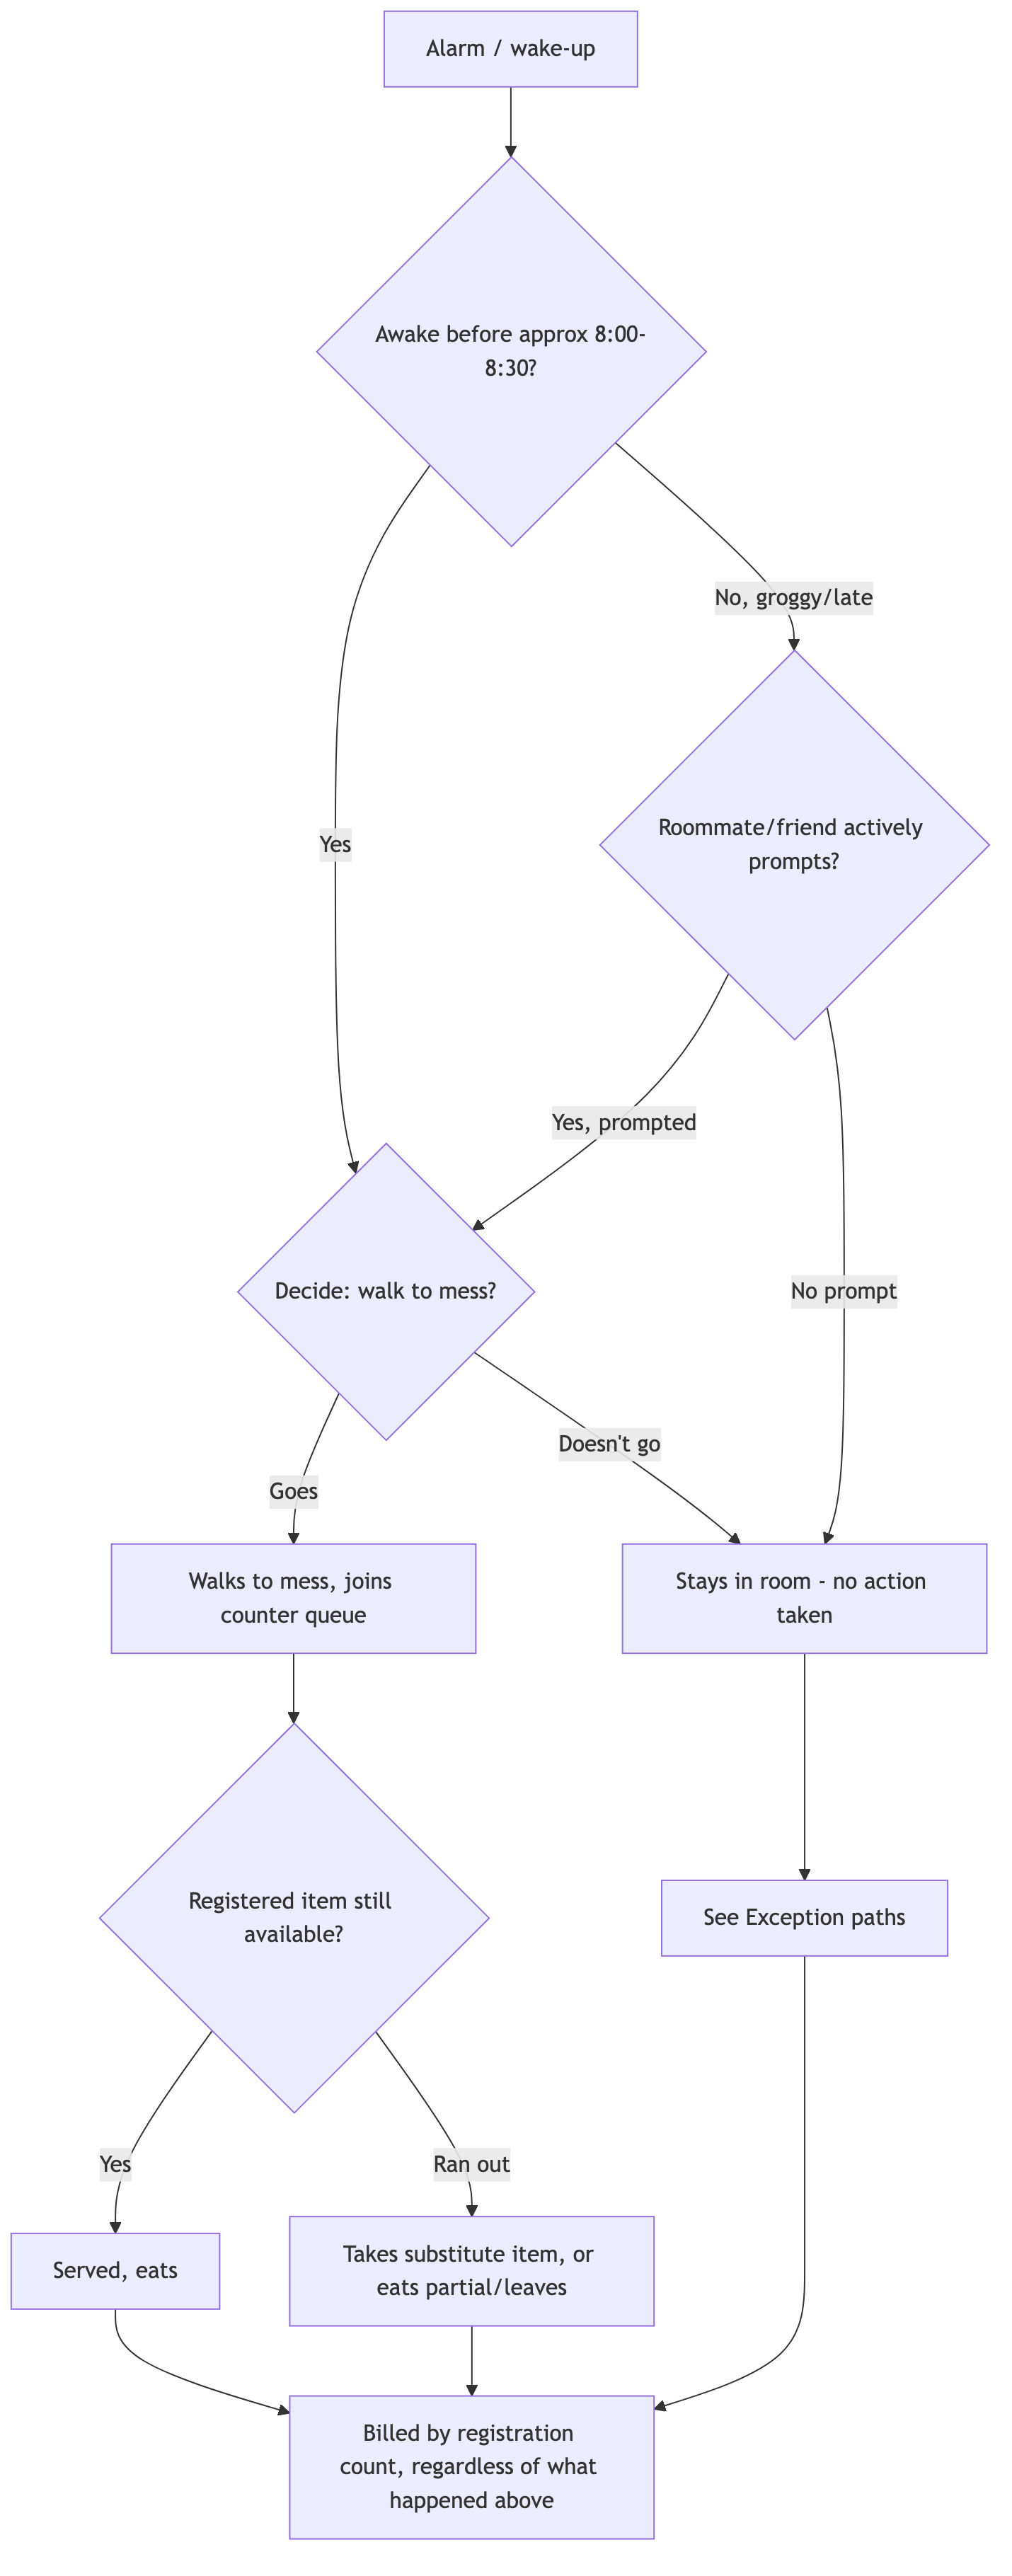
\includegraphics[width=0.95\textwidth]{figures/d8-daily-cycle.png}
    \caption{Daily attendance-decision cycle within the breakfast window.}
\end{figure}

\subsection{C. Exception and Workaround Paths}

\begin{figure}[h]
    \centering
    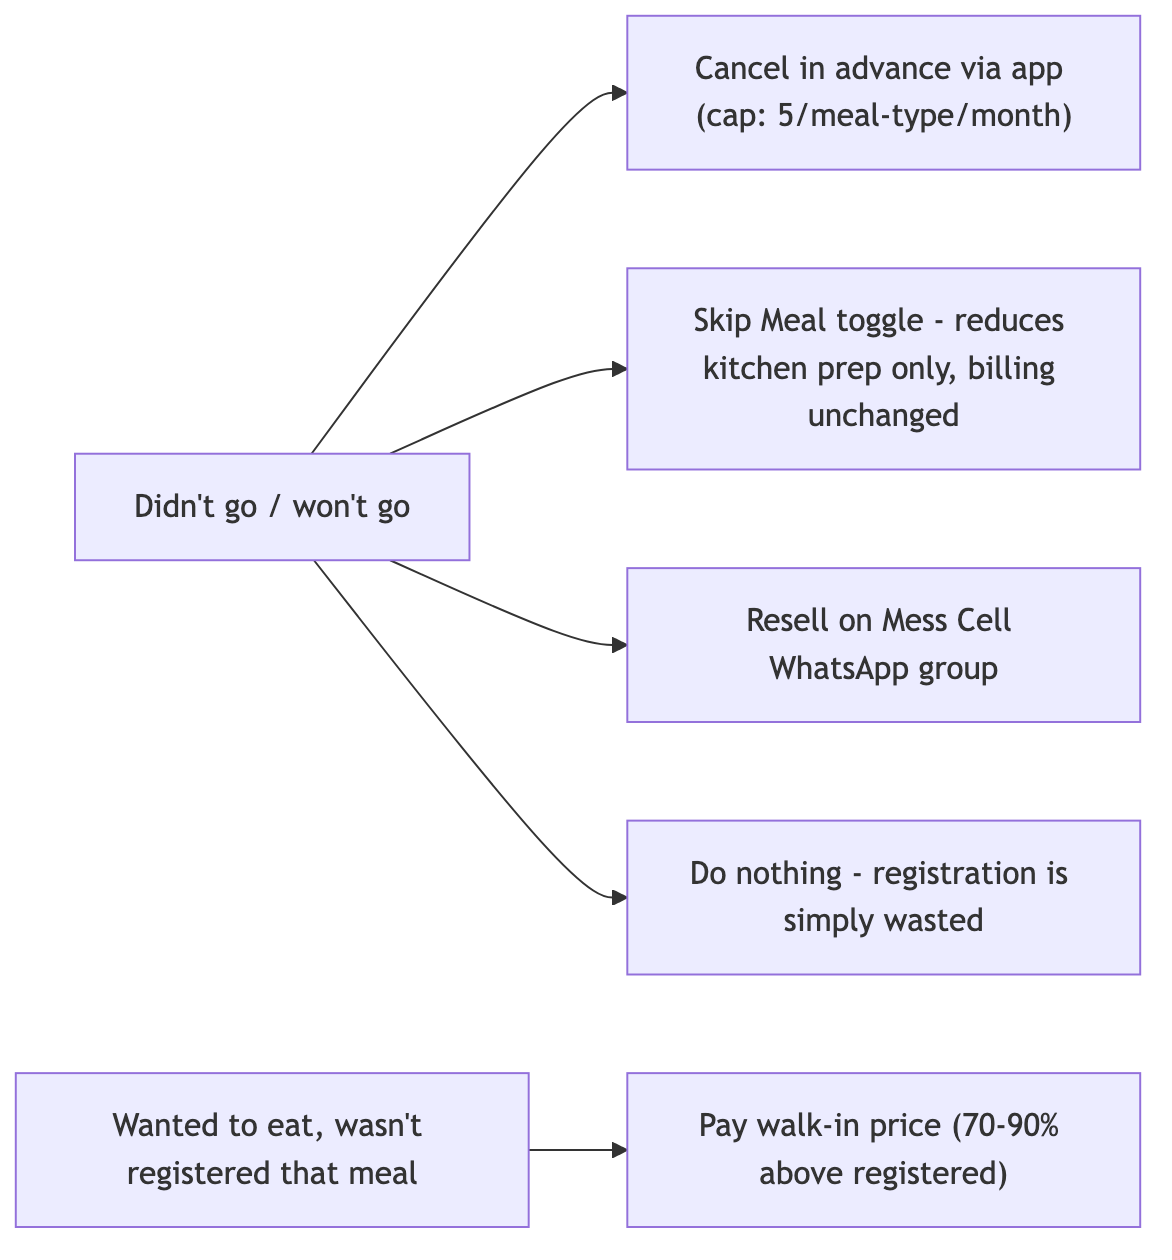
\includegraphics[width=0.85\textwidth]{figures/d9-exception-paths.png}
    \caption{Exception and workaround paths branching off a no-show or an
    unregistered attendance attempt.}
\end{figure}

\subsection{Formal vs.\ Informal Rules Surfaced by This Trace}

\begin{longtable}{L{0.2\textwidth}L{0.35\textwidth}L{0.35\textwidth}}
\toprule
\textbf{Step} & \textbf{Formal rule (as designed)} & \textbf{Informal reality (as it
actually runs)} \\
\midrule
\endhead
Registration & Per-meal opt-in via app & \hypo\ Possibly batched weekly, decoupling
the decision from any single morning \\[6pt]

No-show & Billed regardless \confirmed & A five-per-month cancellation cap exists
specifically because uncancelled no-shows are common enough to need a limit --- the
rule is a symptom of the pattern, not just a control on it \\[6pt]

Kitchen over-preparation & ``Skip Meal'' toggle exists to prevent it \confirmed &
Toggle doesn't touch billing --- solves the kitchen's problem, not the student's \\[6pt]

Unused registration & No official resale/refund mechanism & Mess Cell WhatsApp group
--- fully informal, self-organized, price set peer-to-peer with no oversight
\confirmed\ (exists), \hypo\ (scale) \\[6pt]

Student feedback on rules & Mess Committee ``takes student input'' on menu
\confirmed & No confirmed negotiation or escalation mechanism exists beyond an
occasional feedback form --- a real gap in the trace \\
\bottomrule
\end{longtable}

\subsection{Negotiation and Escalation Mechanisms}

The framework asks this deliverable to identify ``negotiation and escalation
mechanisms.'' Current data has almost none to trace: the Warden handles
vendor/structural changes, the Mess Committee sets the menu ``with student input,''
and that is the extent of any confirmed channel. No respondent so far has described
what a student actually does if they disagree with a mess decision, beyond vague
memories of a petition or feedback form that nobody could confirm led anywhere. This
absence is itself a process-trace finding, worth carrying into the Phase 2 Iceberg
Structures layer as a real gap rather than an unanswered question.

\subsection{What Is Confirmed vs.\ Hypothesized in This Section}

\begin{itemize}
    \item \textbf{\confirmed\ Fully confirmed by the context brief:} billing-by-registration,
        five-per-month cancellation cap, Skip Meal exists and does not affect
        billing, Mess Cell exists, walk-in markup, items running out does happen.
    \item \textbf{\hypo\ Hypothesized, needs a real interview:} batch weekly
        registration, a ``wake-before-8:30 threshold'' effect, a roommate-prompt
        mechanism, Skip Meal being forgotten rather than actively rejected, Mess
        Cell's real transaction scale.
    \item \textbf{Not yet traceable at all:} the mess-side process (kitchen prep
        timing, what staff actually do with unclaimed food) --- entirely dependent on
        the mess-staff (Role C) interview; this section currently only traces the
        student-facing half of the process.
\end{itemize}

\newpage

%============================================================
\section{Task 5: System Timeline / Behaviour-Over-Time Map}
\status{Draft --- direct observation window has already passed for this cycle; this section substitutes existing screenshot data, confirmed context-brief facts, and retrospective recall pending interview confirmation}

Two timescales matter here, and they are kept separate rather than collapsed into one
chart.

\subsection{A. Within-Window Pattern (7:30--9:30 AM, Half-Hour Scale)}
\hypo\ Nothing in this table is measured; it is a plausible curve based on general
dining/class-start dynamics, written down specifically so it can be
\emph{overwritten}, not just annotated, once interview data comes back.

\begin{longtable}{L{0.2\textwidth}L{0.25\textwidth}L{0.45\textwidth}}
\toprule
\textbf{Window} & \textbf{Hypothesized crowd level} & \textbf{Reasoning (to be
tested)} \\
\midrule
\endhead
7:30--8:00 & Moderate & Early-class students and habitual early risers \\
8:00--8:30 & Peak & Closest to the 8:30 class start --- highest queue pressure \\
8:30--9:00 & Dip & Anyone with an 8:30 class has already gone or given up \\
9:00--9:30 & Small second bump & Late risers with no early class, before close \\
\bottomrule
\end{longtable}

\subsection{B. Across-Time Pattern (Week Scale)}

{\small\setlength{\tabcolsep}{4pt}
\begin{longtable}{L{0.12\textwidth}L{0.11\textwidth}L{0.18\textwidth}L{0.36\textwidth}L{0.1\textwidth}}
\toprule
\textbf{Date} & \textbf{Meal} & \textbf{Type} & \textbf{Detail} & \textbf{Source} \\
\midrule
\endhead
2026-09-03 & Breakfast & Individual instance & Respondent's own Kadamba (Veg)
registration, charged \rs 48, not attended & Screenshot \\
2026-09-09 & Breakfast & Mess-wide capacity & Kadamba (Veg) 551/700 registered &
Screenshot \\
2026-09-09 & Breakfast & Mess-wide capacity & Bakul (Veg) 108/350 registered &
Screenshot \\
2026-09-09 & Breakfast & Mess-wide capacity & Bakul (Non-Veg) 37/350 registered &
Screenshot \\
2026-09-10 & Lunch & Mess-wide capacity & Kadamba 722/1200 registered & Screenshot \\
2026-09-10 & Lunch & Mess-wide capacity & Bakul 116/700 registered & Screenshot \\
\bottomrule
\end{longtable}}

\hypo\ Three scattered dates across two different meals is not enough to plot a real
trend line --- a smooth graph through these points would fabricate a precision that
is not there. What this table does consistently support, on every date sampled so
far, is a persistent Kadamba $\gg$ Bakul uptake gap, at both breakfast and lunch.

\subsection{The Recurring Pattern and Unintended Consequence}

This finding does not need a numeric chart to count as a Behaviour-Over-Time result,
and is already fully supported by facts confirmed in Task 1:

\begin{enumerate}
    \item \textbf{Trigger (a structure):} billing is by registration, not attendance.
    \item \textbf{Recurring pattern:} students register and do not show up, often
        enough that a five-cancellations-per-month cap exists --- a cap that only
        makes sense if uncancelled no-shows are common. \confirmed
    \item \textbf{The system's own partial fix, and its unintended consequence:} the
        ``Skip Meal'' toggle exists so kitchens stop over-preparing for known
        no-shows --- but it does not touch billing, so it solves the kitchen's waste
        problem without touching the student's cost problem. \confirmed
    \item \textbf{Emergent adaptation:} the Mess Cell WhatsApp resale market appeared,
        unofficially, as a workaround the system's designers did not build for.
        \confirmed
\end{enumerate}

This reinforcing-loop-shaped structure feeds directly into the Phase 2 Causal Loop
Diagram deliverable.

\subsection{Feedback Loops and Systems Archetypes}

\subsubsection*{Quick Iceberg pass}

\begin{itemize}
    \item \textbf{Events:} the September 3 charged-not-attended instance; items
        running out near the end of service; Kadamba sitting near capacity while
        Bakul sits far under it.
    \item \textbf{Patterns:} registration consistently exceeds attendance (the cap
        exists because of this); Kadamba $\gg$ Bakul uptake on every date sampled, at
        both meals.
    \item \textbf{Structures:} billing-by-registration; the five-per-month
        cancellation cap; Skip Meal (a kitchen-only fix); the informal Mess Cell
        market; \hypo\ possible batch-weekly registration; no confirmed escalation
        channel.
    \item \textbf{Mental models (all \hypo, none directly confirmed yet):} ``I
        already paid for it, the money's gone either way''; ``giving feedback
        doesn't really change anything''; ``Kadamba is just the trusted default.''
\end{itemize}

\subsubsection*{R1 --- ``Shifting the Burden'' via Mess Cell}
Reinforcing --- sustains the dysfunction rather than growing it unboundedly.

\begin{figure}[h]
    \centering
    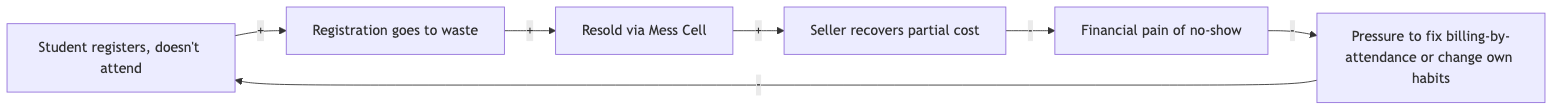
\includegraphics[width=0.85\textwidth]{figures/d10-loop-r1.png}
    \caption{R1: the Mess Cell resale market as a Shifting the Burden loop.}
\end{figure}

The informal resale market is a symptomatic relief valve that makes the underlying
problem (billing does not track attendance) tolerable enough that nobody --- student,
Mess Committee, or Warden --- is ever forced to fix the fundamental cause. The
workaround's success is exactly what lets the root cause persist.

\subsubsection*{B1 --- Kitchen Waste Control}
Balancing, but only for half the problem --- a Fix That Fails.

\begin{figure}[h]
    \centering
    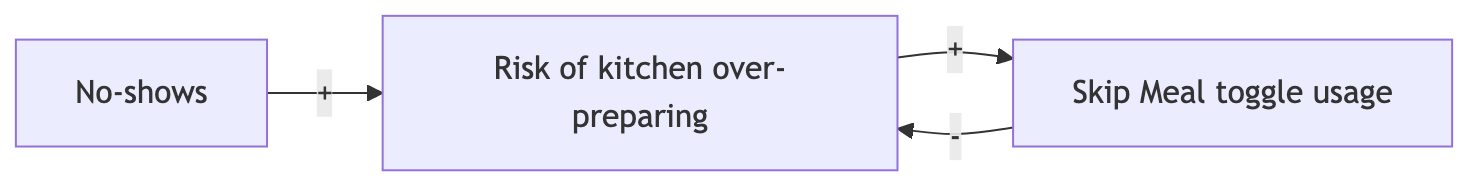
\includegraphics[width=0.6\textwidth]{figures/d11-loop-b1.png}
    \caption{B1: Skip Meal balances kitchen over-preparation, but not billing.}
\end{figure}

This loop genuinely balances --- it is why the toggle exists --- but it only closes
the kitchen-side variable. Billing (the student-side variable) has no corresponding
balancing loop at all, which is precisely why B1 reads as a Fix That Fails: it looks
like the no-show problem was addressed, which may reduce the perceived urgency of
fixing the billing model, even though the student's actual cost problem is untouched.

\subsubsection*{Systems archetypes mapped onto current data}

\begin{itemize}
    \item \textbf{Fixes that Fail} --- Skip Meal: solves kitchen waste, leaves
        billing broken, possibly reduces pressure to fix the real issue.
    \item \textbf{Shifting the Burden} --- Mess Cell resale: symptomatic relief
        substituting for structural reform.
    \item \textbf{Limits to Growth} --- \confirmed\ already happened once: Kadamba
        hit a capacity ceiling on non-veg demand, and Bakul was created as the
        workaround. \openq\ Has the limiting factor now shifted from kitchen
        capacity to student preference/trust, since Bakul has spare capacity but
        still is not chosen?
    \item \textbf{Tragedy of the Commons} --- \hypo\ the shared counter/kitchen
        throughput during the 8:00--8:30 peak is a commons everyone draws on by
        timing their arrival right before class, degrading queue speed for everyone,
        with no individual student bearing the cost of their own contribution to it.
        Needs a staff perspective to confirm.
    \item \textbf{Overoptimization} --- billing-by-registration-count optimizes for
        administrative simplicity and kitchen-planning predictability, at the direct
        expense of matching food produced to food eaten and cost to value received.
    \item \textbf{Ignoring stakeholders} --- the Academic Office (holds the one lever
        most likely to help, zero engagement) and mess staff (day-to-day operational
        knowledge with no confirmed channel upward).
    \item \textbf{Manipulating/gaming the system} --- the Mess Cell market itself is
        a mild gaming behavior: extracting value from a system not designed for
        resale. \openq\ Is this mostly accidental no-shows recovered after the fact,
        or do some students deliberately register broadly intending to resell what
        they don't use? These are different diagnoses --- a design flaw producing
        waste, versus a rational response to a mispriced system.
\end{itemize}

\subsubsection*{A weak/broken balancing loop worth naming}

\textbf{B2 --- Capacity Redistribution (designed to work, doesn't appear to):} the
natural balancing response to Kadamba nearing capacity should be organic
redistribution to Bakul/Palash. Observed data shows this is not happening --- Kadamba
runs near 79\% of printed capacity while Bakul sits at 31\%/11\% (veg/non-veg) on
the one date sampled. Instead of the loop self-correcting, capacity was added
administratively (Bakul was built). Why the organic loop does not work --- awareness,
preference, or the ``trusted default'' mental model above --- remains a real open
question, not an assumption.

\newpage

%============================================================
\section{Summary and Status}

{\small\setlength{\tabcolsep}{4pt}
\begin{longtable}{L{0.06\textwidth}L{0.32\textwidth}L{0.19\textwidth}L{0.31\textwidth}}
\toprule
\textbf{\#} & \textbf{Deliverable} & \textbf{Status} & \textbf{What closes remaining gaps} \\
\midrule
\endhead
1 & System Context Brief & Complete & --- \\[4pt]
2 & Stakeholder Map & Complete & --- \\[4pt]
3 & Stakeholder Power--Interest / Leverage Map & Draft, finalizing & Governance
(Role D) interview confirms the Academic Office / vendor power reads \\[4pt]
4 & Current-State Process Map / Process Trace & Draft, pending fieldwork & Student
(Role A/B) and mess-staff (Role C) interviews confirm the weekly-batching,
roommate-prompt, and kitchen-side hypotheses \\[4pt]
5 & System Timeline / Behaviour-Over-Time Map & Draft, pending fieldwork & Same
interviews replace the within-window hypothesis table with real recalled or observed
data \\
\bottomrule
\end{longtable}}

Everything that could be built from existing confirmed facts and structural
reasoning is done. The two remaining gaps are exactly where the framework itself
requires real human input: Activity 4's ``conduct interviews and observations'' and
Activity 5's ``collect historical... observations.'' Both are being closed through
the ongoing round of Role A (attending students), Role B (skipping students), Role C
(mess operations staff), and Role D (mess governance) interviews. This report will be
updated in place as each round of interview data lands.

\end{document}
